\section{Integral- und Flächenberechnung}
\subsection{Einführung - Treppensummen}
\subsubsection{Flächenberechnung}
\begin{frame}{Integral konstanter Funktionen}
	Arbeit ist physikalisch definiert als Kraft mal Weg, also für eine konstante Kraft $F(x)=F$
	\[
		W=F \cdot (x_{2} - x_{1}) 
	\]
	wenn $x_{1}$ und $x_{2}$ der Start- und der Endpunkt des Weges sind, über den die Kraft $F$ ausgeübt wird. Das entspricht aber der Fläche zwischen dem Funktionsgraphen und der $x$-Achse zwischen den Stellen $x_{1}$ und $x_{2}$
	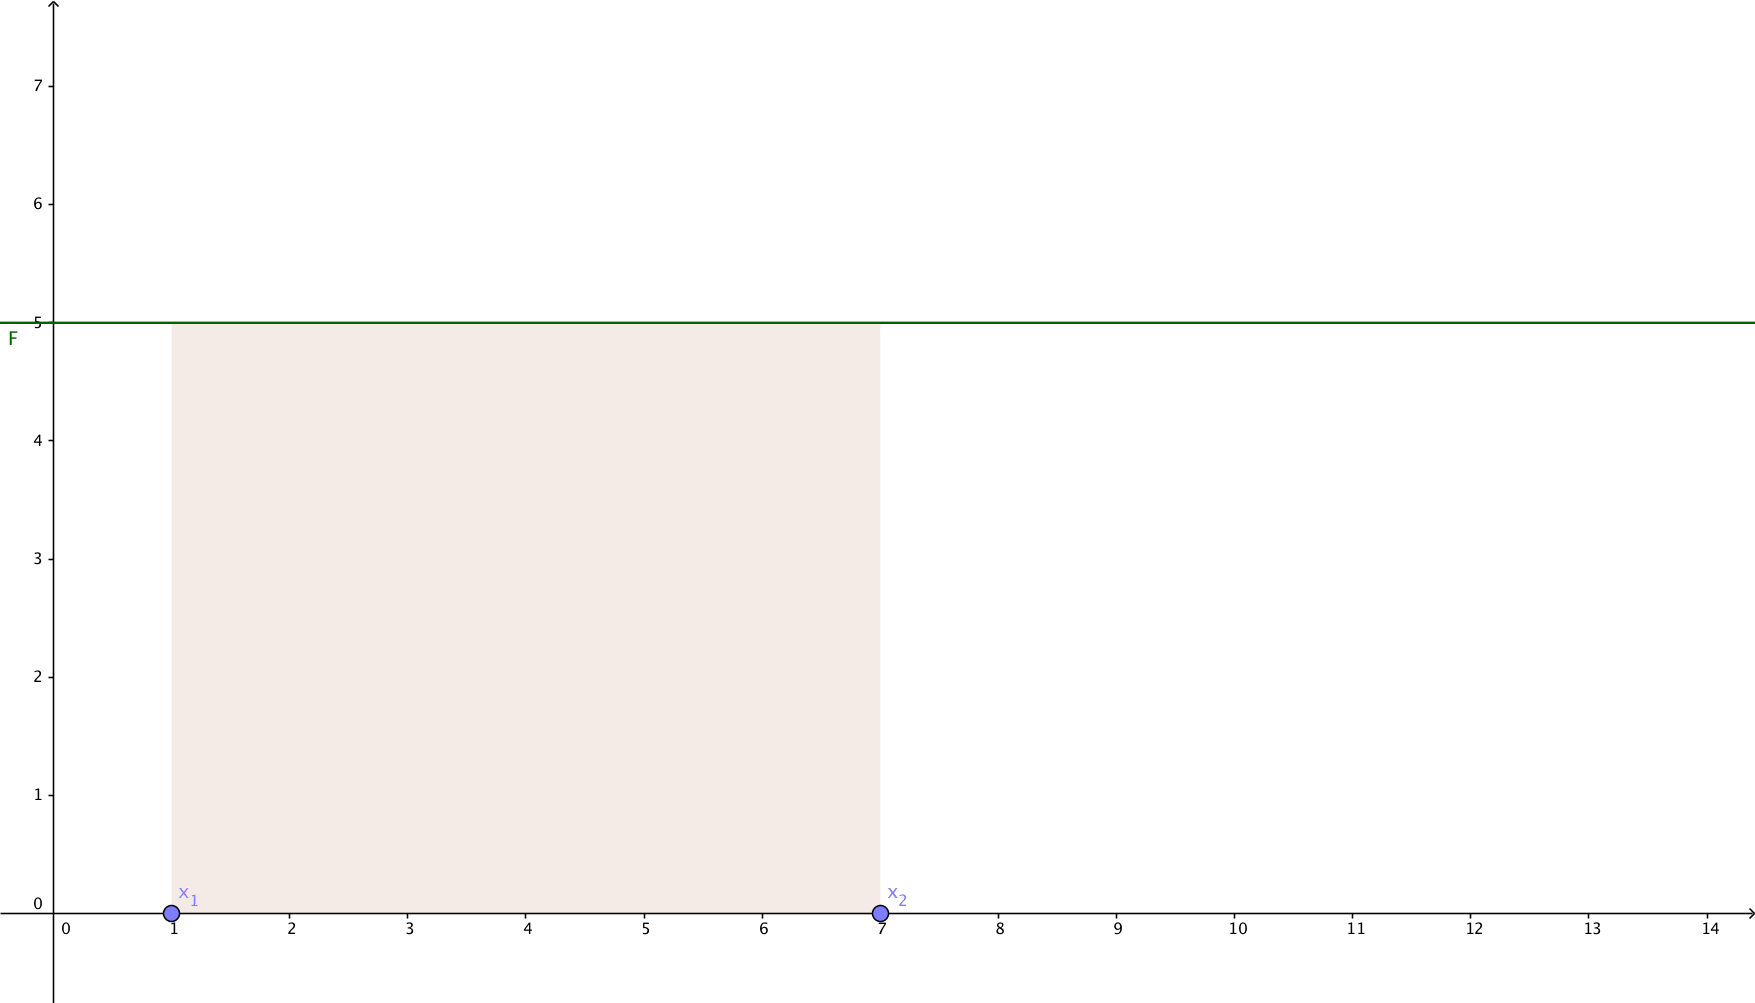
\includegraphics[width=8cm]{integral_konstantefunktion}
\end{frame}

\begin{frame}{Integral linearer Funktionen}
	Für eine nicht-konstante, aber lineare vom Weg abhängige Kraft $F(x)=a \cdot x + b$ ist die Berechnung der Arbeit schon etwas schwieriger, weil nun die Kraft vom (momentanen) Ort abhängt:
	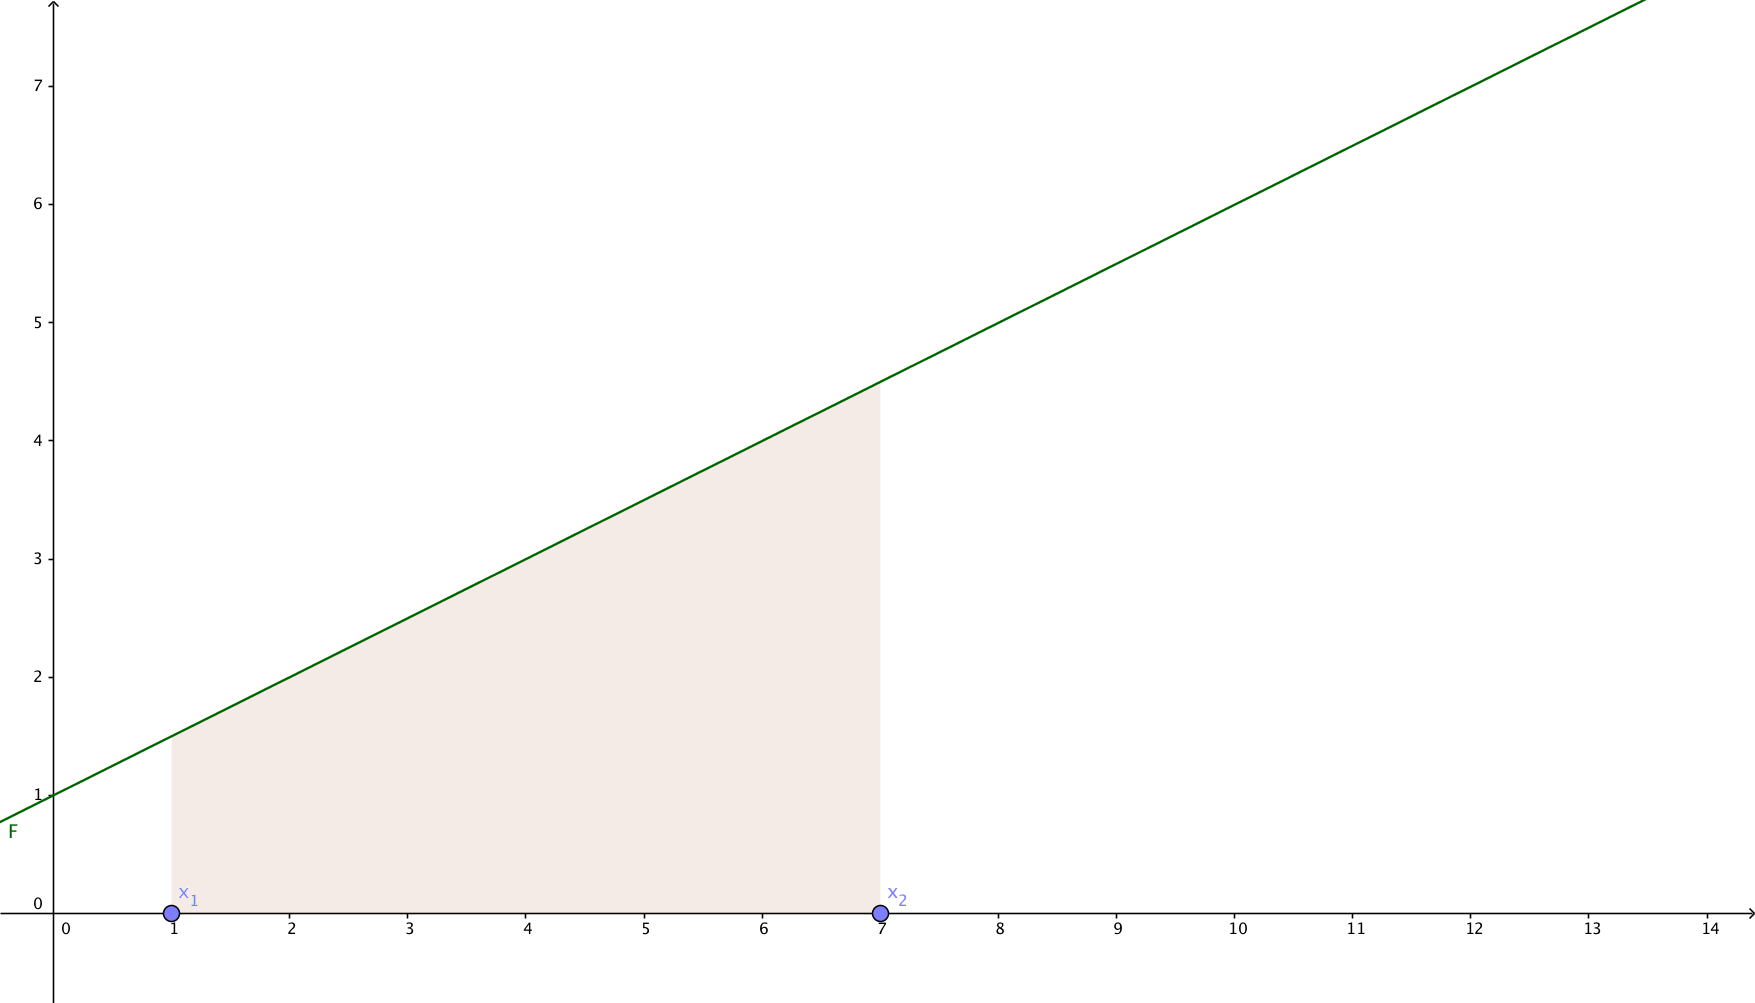
\includegraphics[width=8cm]{integral_linearefunktion}
	
	Geometrisch (Trapezformel) findet man hier:
\scriptsize{	\[
		W = \frac{1}{2} (F(x_{2})+F(x_{1})) (x_{2}-x_{1}) = \frac{1}{2} (ax_{2} + b + (ax_{1} + b)) (x_{2}-x_{1}) = ax_{2}^2-ax_{1}^{2} + b(x_{2}-x_{1})
	\]}
\end{frame}

\begin{frame}{Integral quadratische Funktion}
	\tiny{
	Für die quadratische Funktion $F(x)=x^{2}$ wir das ganze komplizierter, daher verwenden wir hier $N$ einfache (untere) Treppenfunktionen:
	
	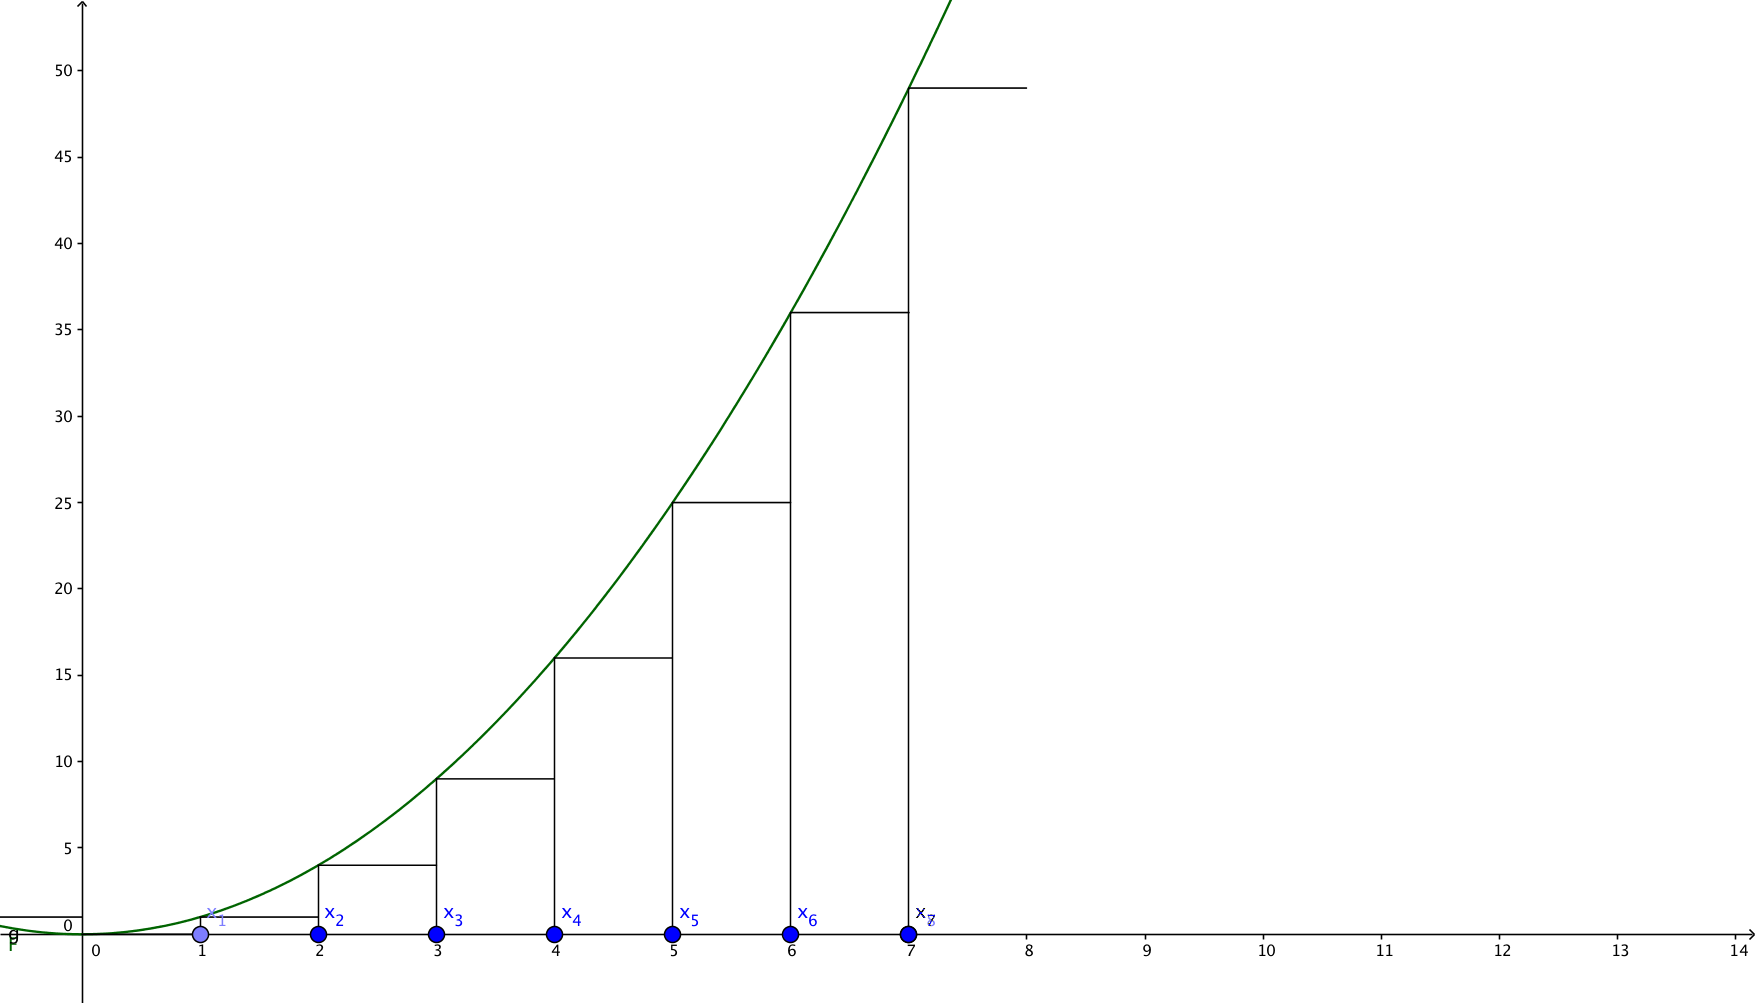
\includegraphics[width=8cm]{integral_quadratischefunktion}

	Für jedes einzelne Rechteck ($k=1, \ldots 6$) gilt mit $(x_{k+1} - x_{k}) = \frac{b-a}{N}$, wobei $a=x_{1}$ und $b=x_{N+1}$ ist:
	\begin{align*}
		W_{N}^{U}(k) & = F(x_{k}) \cdot (x_{k+1} - x_{k}) = F(x_{k}) \cdot \frac{b-a}{N} \\
		& = F\left((k-1)\frac{b-a}{N} + a\right) \frac{b-a}{N} \\
		& = \left( (k-1)^2\frac{(b-a)^2}{N^2} + 2(k-1) \frac{b-a}{N}a + a^2 \right) \frac{b-a}{N}
	\end{align*}}
\end{frame}

\begin{frame}{Integral quadratische Funktion}
\small{	Damit gilt für die gesamte Fläche (näherungsweise)
	\begin{align*}
		W_{N}^{U} & = \sum_{k=1}^{N} W(k) = \sum_{k=1}^{N} (k-1)^2 \frac{(b-a)^3}{N^3} + 2(k-1)\frac{(b-a)^2}{N^2}a + a^2 \frac{b-a}{N} \\
		&  = \sum_{k=0}^{N-1} k^2 \frac{(b-a)^3}{N^3} + 2k\frac{(b-a)^2}{N^2}a + a^2 \frac{b-a}{N} \\
		& = \frac{(b-a)^3}{N^3} \left( \sum_{k=0}^{N-1} k^2 \right)  + 2\frac{(b-a)^2}{N^2}a \left( \sum_{k=0}^{N-1} k \right) + a^2 (b-a) \\
		& = \frac{(b-a)^3}{N^3} \frac{N(N-1)(2N-1)}{6}  + 2\frac{(b-a)^2}{N^2}a \frac{N(N-1)}{2} + a^2 (b-a) \\
		& = \frac{(b-a)^3}{6N^3} \left( 2N^3 - 3N^2 + N \right) + \frac{(b-a)^2}{N^2} a (N^2 - N) +a^2 (b-a)
	\end{align*}
	Für $N \to \infty$ ist das
	\begin{align*}
		\lim_{N \to \infty} W_{N}^{U} & = \frac{(b-a)^3}{3} + (b-a)^2 a + a^2 (b-a) \\
		& = \frac{1}{3}b^3 - \frac{1}{3} a^3
  	\end{align*}}
\end{frame}

\begin{frame}{Grenzwerte oberer und unterer Treppenfunktionen}
	Für die untere Treppenfunktion gilt also:
	\[
		\lim_{N \to \infty} W_{N}^{U} = \frac{1}{3} b^3 - \frac{1}{3}a^3
	\]
	Entsprechend (ersetze $k-1$ durch $k$) gilt für die obere Treppenfunktion:
		\[
		\lim_{N \to \infty} W_{N}^{O} = \frac{1}{3} b^3 - \frac{1}{3}a^3
		\]
		
	Das heißt, die Fläche unter der Funktion $F(x)=x^2$ zwischen den Grenzen $a$ und $b$ ist $\frac{b^3 - a^3}{3}$.
\end{frame}

\subsection{Bestimmte Integrale}
\begin{frame}{Bestimmte Integrale}
	
	\begin{bemerkung}
		In der ausführlichen Rechnung tauchen immer fünf Dinge auf:
		\begin{itemize}
			\item ein Grenzwert ($N \to \infty$).
			\item ein Summenzeichen ($\sum_{k=1}^{N}$)
			\item die äußersten Grenzen $a$ und $b$
			\item die Funktionswerte an den Rechteckgrenzen (rechts oder links) $f(x_{k})$ bzw. $f(x_{k+1})$
			\item Die Breite der Rechtecke ($\Delta x_{k} = x_{k+1} - x_{k} = \frac{b-a}{N}$)
		\end{itemize}
		Also eigentlich ein Ausdruck der Form
		\[
			\lim_{N \to \infty}\sum_{k=1}^{N} F(x_{k}) \Delta x_{k}
		\]
	\end{bemerkung}
\end{frame}	
\begin{frame}{Stammfunktion}
	\begin{definition}
		Den o.g. Grenzwert bezeichnet man als \textbf{das bestimmte Integral von $f$ zwischen $a$ und $b$} und schreibt:
		\[
			\int_{a}^{b} f(x) dx
		\]
	\end{definition}
	\begin{definition}
		Definiert man die Funktion $F$ als
		\[
			F(x):=\int_{a}^{x} f(x) dx
		\]
		so erhält man eine \textbf{Integralfunktion} oder \textbf{Stammfunktion} von $f$.
		Insbesondere ist 
		\[
			\int_{0}^{x} x^2 dx = \frac{1}{3} x^3
		\] 
	\end{definition}
\end{frame}

\begin{frame}{Stammfunktionen und bestimmte Integrale}
	\begin{bemerkung}
		Hat man irgendeine Stammfunktion $F(x)$ zur Funktion $f(x)$ bestimmt, so ist für das bestimmte Integral
		\[
			\int_{a}^{b} f(x) dx = F(b) - F(a)
		\]
		Anschaulich bedeutet das, dass die Fläche zwischen den Grenzen $a$ und $b$ die Differenz derjenigen Fläche zwischen irgendeinem Wert $c$ und $b$ und der Fläche zwischen diesem Wert $c$ und $a$ ist.
		
		Man schreibt dann auch:
		\[
		\int_{a}^{b} f(x) dx = [F(x)]_{a}^{b} = F(x) |_{a}^{b} = F(b) - F(a)	
		\] 
		und bezeichnet $a$ als \textbf{untere Integrationsgrenze} und $b$ als \textbf{obere Integrationsgrenze}.
	\end{bemerkung}
\end{frame}

\begin{frame}{Geometrie des Integrals}
	\begin{bemerkung}
		Geometrisch ist das bestimmte Integral die Fläche zwischen den Grenzen $a$ und $b$, die die Funktion $f$ mit der x-Achse einschließt.
		
		Allerdings werden Flächenteile unterhalb der x-Achse negativ berechnet. Man muss also für die tatsächliche Fläche auf Vorzeichenwechsel der Funktion $f$ achten.
	\end{bemerkung}
\end{frame}

\subsection{Unbestimmte Integrale}

\begin{frame}{Unbestimmte Integrale}
	\begin{bemerkung}
		Hat man eine Stammfunktion $F(x)$ zur Funktion $f(x)$ bestimmt, so ist für jede konstante $C$ auch die Funktion $F_{C}(x) := F(x) + C$ eine Stammfunktion von $f(x)$, denn
		\[
			F_{C}'(x) = F'(x) = f(x)
		\]
		Es gibt also zu einer Funktion $f(x)$ unendlich viele Stammfunktionen.
		Da es egal ist, welche Stammfunktion man für die Berechnung der bestimmten Intgrale verwendet, bezeichnet man 
		\[
			\int f(x) dx = F(x) + C
		\]
		als das \textbf{unbestimmte Integral} der Funktion $f(x)$.
		Je zwei Stammfunktionen $F_{1}(x)$ und $F_{2}(x)$ zu einer Funktion $f(x)$ können sich höchstens um eine Konstante unterscheiden, weil
		\[
			F_{1}'(x) - F_{2}'(x) = f(x) - f(x) = 0
		\]
	\end{bemerkung}
\end{frame}

\subsection{Elementare Stammfunktionen}

\begin{frame}{Elementare Stammfunktionen}
\footnotesize{
	\begin{example}
		\begin{align*}
			\int 2x dx & = x^2 +C \\
			\int \frac{1}{2\sqrt{x}} dx & = \sqrt{x} + C \\
			\int \frac{1}{x} dx & = \ln |x| + C \\
			\int e^{x} dx & = e^{x} + C \\
			\int x^{\alpha} dx & = \frac{1}{\alpha + 1} x^{\alpha + 1} + C \qquad \forall \alpha \in \mathbb{R} \setminus \{ -1 \} \\
			\int a^{x} dx & = \frac{1}{\ln a} a^{x} + C \\
			\int \sin (x) dx & = - \cos (x) + C \\
			\int \cos (x) dx & = \sin (x) +C \\
			\int \frac{1}{1+x^{2}} dx & = \arctan x + C
		\end{align*}	
	\end{example}}
\end{frame}

\subsection{Integrationsregeln}

\begin{frame}{Integrationsregeln}
	\begin{bemerkung}
		So, wie es für die Ableitung bestimmte Regeln und Sätze gibt, die angeben, wie man die Ableitung zusammengesetzter Funktionen berechnen kann, gibt es Regeln für die Bestimmung von Integralen. 
		
			Wir werden uns im Folgenden mit diesen Regeln befassen:
			\begin{itemize}
				\item Faktorregel
				\item Summen- und Differenzenregel
				\item Partielle Integration
				\item Integration durch Substitution
				\item Logarithmische Integration
				\item Partialbruchzerlegung
			\end{itemize}
	\end{bemerkung}
\end{frame}

\subsection{Faktor-, Summen- und Differenzenregel}
\begin{frame}{Faktor-, Summen- und Differenzenregel}
	\begin{theorem}
		Für das (un-)bestimmte Integral zweier Funktionen $f(x)$ und $g(x)$ gilt:
		\begin{align*}
			\int k f(x) dx & = k \int f(x) dx \qquad \forall k \in \mathbb{R} & \text{  Faktorregel} \\
			\int f(x) + g(x) dx & = \int f(x) dx + \int g(x) dx & \text{  Summenregel}\\
			\int f(x) - g(x) dx & = \int f(x) dx - \int g(x) dx & \text{  Differenzenregel}\\
		\end{align*}
		Die Faktor- und die Summenregel fasst man auch zusammen unter dem Begriff der \textbf{Linearität des Integrals}
	\end{theorem}
\end{frame}

\begin{frame}{Intervallzerlegung}
	\begin{bemerkung}
		Für $a \leq b \leq c$ und eine integrierbare Funktion $f$ gilt:
		\[
			\int_{a}^{c} f(x) dx = \int_{a}^{b} f(x) dx + \int_{b}^{c} f(x) dx
		\]
		
		Für die Fläche $A$ zwischen x-Achse und der Funktion $f(x)$ gilt:
		\begin{align*}
			A = \int_{a}^{b} f(x) dx \geq 0 & \text{ falls } f(x) \geq 0 \qquad\forall x\in [a, b] \\
			A = - \int_{a}^{b} f(x) dx \geq 0 & \text{ falls } f(x) \leq 0 \qquad \forall x\in [a, b]
		\end{align*}
	\end{bemerkung}
\end{frame}

\begin{frame}{Symmetrieeigenschaften des Integrals}
	\begin{bemerkung}
		Für eine gerade Funktion $f(x)$ (also $f(-x) = f(x) \quad \forall x$) gilt:
		\[
			\int_{-a}^{a} f(x) dx = 2 \int_{0}^{a} f(x) dx
		\]

		Für eine ungerade Funktion $f(x)$ (also $f(-x) = -f(x) \quad \forall x$) gilt:
		\[
			\int_{-a}^{a} f(x) dx = 0
		\]
		
		Für das bestimmte Integral gilt allgemein:
		\begin{align*}
			\int_{a}^{b} f(x) dx & = - \int_{b}^{a} f(x) dx \\
			\left| \int_{a}^{b} f(x) dx \right| & \leq \int_{a}^{b} | f(x) | dx
		\end{align*}

	\end{bemerkung}
\end{frame}

\subsection{Partielle Integration}

\begin{frame}{Partielle Integration}
\begin{bemerkung}
	Für die Ableitung einer differenzierbaren Funktion $h(x)=f(x)\cdot g(x)$ gilt die Produktregel:
	\[
		h'(x) = (f\cdot g)'(x) = f'(x)\cdot g(x) + f(x) \cdot g'(x) 
	\]
	Das bedeutet für die Funktion $h$ als Stammfunktion von $h'$ 
	\small{\begin{align*}
		& \int_{a}^{b} h'(x) dx = \left[ (f(x) \cdot g(x)) \right]_{a}^{b} = \int_{a}^{b} f'(x) \cdot g(x) dx + \int_{a}^{b} f(x)\cdot g'(x) dx \\
		& \Leftrightarrow \int_{a}^{b} f(x)\cdot g'(x) dx = [f(x)\cdot g(x)]_{a}^{b} - \int_{a}^{b} f'(x)\cdot g(x) dx
 	\end{align*}}
\end{bemerkung}
\end{frame}

\begin{frame}{Partielle Integration}
\begin{theorem}[Partielle Integration]
	Für das bestimmte Integral gilt:
	\[
		\int_{a}^{b} f(x)\cdot g'(x) dx = f(x)\cdot g(x) |_{a}^{b} - \int_{a}^{b} f'(x) \cdot g(x) dx
	\]
	
	Für das unbestimmte Integral gilt entsprechend:
	\[
		\int f(x)\cdot g'(x) dx = f(x)\cdot g(x) - \int f'(x) \cdot g(x) dx
	\]
\end{theorem}
\begin{bemerkung}
	Der Satz ist dann nützlich, wenn man das Produkt zweier Funktionen integrieren möchte und die Stammfunktion $g(x)$ des einen Faktors (hier $g'(x)$) kennt. Man wälzt dann mit diesem Satz die Ableitung des Fakt $g'(x)$ auf $f(x)$; oft vereinfacht das die Integration. 
\end{bemerkung}
\end{frame}

\begin{frame}{Beispiele zur partiellen Integration}
	\begin{example}
		Für die Stammfunktion der Funktion $h(x)=x\cdot e^{x}$ gilt mit $f(x)=x$ und $g'(x)=e^{x}$:
		\begin{align*}
			\int x e^{x} dx & = x \cdot e^{x} - \int 1 \cdot e^{x} dx = x \cdot e^{x} - e^{x} + C = (x-1) \cdot e^{x} + C
 		\end{align*}
	\end{example}
	\begin{example}
		Für die Stammfunktion der Funktion $h(x)=x^{2} \cdot \ln x$ gilt mit $f'(x)=x^{2}$ und $g(x)=\ln x$:
		\begin{align*}
			\int x^2 \ln x dx & = \frac{1}{3}x^{3} \cdot \ln x - \int \frac{1}{3}x^{3} \cdot \frac{1}{x}dx \\ 
				& = \frac{1}{3}x^{3} \ln x - \frac{1}{3} \int x^{2} dx \\ 
				& = \frac{1}{3}x^{3} \ln x - \frac{1}{9} x^{3} + C
 		\end{align*}
	\end{example}
	
\end{frame}

\begin{frame}{Beispiele zur partiellen Integration}
\begin{example}
	Für die Stammfunktion der Funktion $h(x)=(3x-7)\cdot e^{-x}$ gilt mit $f(x)=3x+7$ und $g'(x)=e^{-x}$:
		\begin{align*}
			\int (3x-7) \cdot e^{-x} dx & = (3x-7)\cdot (-e^{-x}) - \int 3 \cdot (-e^{-x}) dx \\
			& = (3x-7)\cdot (-e^{-x}) + 3 \int e^{-x} dx \\
			& = (3x-7)\cdot (-e^{-x}) - 3 e^{-x} + C\\
			& = (4-3x)\cdot e^{-x} +C
		\end{align*}
\end{example}
\end{frame}

\begin{frame}{Beispiele zur partiellen Integration}
\begin{example}
	Für die Stammfunktion der Funktion $h(x)=x \cos x$ gilt mit $f(x)=x$ und $g'(x)=\cos x$:
	\begin{align*}
		\int x \cos x \, dx & = x \sin x - \int 1 \cdot \sin x \, dx \\
		& = x \sin x + \cos x + C 
	\end{align*}
\end{example}
\end{frame}

\begin{frame}{Beispiele zur partiellen Integration}
\small{	
	\begin{example}
		Für das Integral der Funktion $h(x)= \sin^{2} x$ gilt mit $f(x)=\sin x$ und $g'(x)= \sin x$:
		\begin{align*}
			\int \sin^{2} x \, dx & = \int \sin x \cdot \sin x \, dx = -\sin x \cdot \cos x + \int \cos x \cdot \cos x \, dx \\
			& = -\sin x \cdot \cos x + \int \cos^{2} x \, dx \\ 
			& = -\sin x \cdot \cos x + \int 1-\sin^{2} x \, dx\\
			& = -\sin x \cdot \cos x + x - \int \sin^{2} x \, dx \\
			\Leftrightarrow 2\cdot \int \sin^{2} x\, dx & = -\sin x \cdot \cos x + x \\
			\Leftrightarrow  \int \sin^{2} x\, dx & = -\frac{1}{2}\sin x \cdot \cos x + \frac{x}{2}
		\end{align*}
	\end{example}}
\end{frame}

\subsection{Integration durch Substitution}
\begin{frame}{Integration durch Substitution}
\begin{bemerkung}
\footnotesize{	Die Kettenregel für die Ableitung einer Funktion $h(x)=f(g(x))$ lautet:
	\[
		h'(x) = f'(g(x)) \cdot g'(x)
	\]
	Wir hatten das auch mal so geschrieben:
	\[
		\frac{dh}{dx}(x) = \frac{df}{dg}(g(x)) \cdot \frac{dg}{dx}(x)
	\]
	oder noch einfacher (wenn man nicht vergisst, an welchen Stellen man die Funktionen auswertet):
	\[	
		\frac{dh}{dx} = \frac{df}{dg} \cdot \frac{dg}{dx}
	\]
	Integriert man das, so erhält man
	\begin{align*}
		\int \frac{dh}{dx} dx  & = \int \frac{df}{dg} \cdot \frac{dg}{dx} dx \\
		\Leftrightarrow h(x) & = \int \frac{df}{dg} \cdot dg = f(g) = f(g(x))
	\end{align*}
	Es genügt also in diesem Fall, die Stammfunktion $f$ als Funktion von $g$ zu kennen. }
\end{bemerkung}
\end{frame}

\begin{frame}{Integration durch Substitution}
\begin{bemerkung}
	Sind $f$ und $g$ stetige Funktionen und $F$ eine Stammfunktion von $f$, so gilt offenbar nicht nur $F'(x)=f(x)$, sondern (wegen der Kettenregel) auch:
	\[
		\left(F(g(x)\right)' = F'(g(x))\cdot g'(x) = f(g(x))\cdot g'(x)
	\]
	Also ist $F(g(x))$ eine Stammfunktion von $f(g(x))\cdot g'(x)$
\end{bemerkung}
\begin{theorem}
	Ist $f(x)$ stetig und $g(x)$ eine stetig differenzierbare, umkehrbare Funktion, dann gilt:
	\[
		\int_{a}^{b} f(x) dx = \int_{g^{-1}(a)}^{g^{-1}(b)} f(g(t)) g'(t) dt = \int_{g^{-1}(a)}^{g^{-1}(b)} f(g) dg
	\]
	Wichtig ist, dass sich auch die Integrationsgrenzen ändern, weil man ja die Integrationsvariable ersetzt hat.
\end{theorem}
\end{frame}


\begin{frame}{Beispiele - Integration durch Substitution}
\begin{example}
Für das Integral
\[
	\int \frac{1}{x+a}dx
\]	
erhält man mit $g(x)=x+a$ und $\frac{dg}{dx}=1$, also $dg=dx$ und daher
\[
\int \frac{1}{x+a}dx = \int \frac{1}{g} dg = \ln |g| + C= \ln |x+a| +C
\]
\end{example}
\begin{example}
	Für das Integral $\int \frac{2x}{x^2+1} dx$ erhält man mit $g(x)=x^2+1$ und $\frac{dg}{dx}= 2x$, also $dg = 2x\,dx$ dann
	\[
		\int \frac{2x}{x^2+1} dx = \int \frac{1}{g}dg = \ln |g| + C = \ln |x^2+1| +C
	\]
\end{example}
\end{frame}

\begin{frame}{Beispiel - Integration durch Substitution}
\begin{example}
	Für das Integral $\int x \cos (x^{2})\,dx$
	\begin{itemize}
		\item substituiert man zuerst $g(x)=x^{2}$, also $x=\sqrt{g}$. Aus dem Integranden wird damit 
			\[
				x \cos (x^{2}) \rightarrow \sqrt{g} \cos (g)
			\]
			\item und für das Differential $dx$ ersetzt man 
			\[
				\frac{dg}{dx} = 2x \quad \Leftrightarrow \quad dx = \frac{dg}{2x} = \frac{dg}{2\sqrt{g}} 
			\]
		\item Für das Integral schreibt man dann also
		\[
			\int x \cos (x^{2}) dx = \int \sqrt{g} \cos (g) \frac{dg}{2 \sqrt{g}} = \frac{1}{2}\int \cos (g) dg = \frac{1}{2}\sin(x^{2})
		\]
	\end{itemize}
\end{example}
\end{frame}


\begin{frame}{Beispiel - Integration durch Substitution}
\begin{example}
	Da $\tan x = \frac{\sin x}{\cos x}$ ist, kann man mit $g(x)=\cos x$ und $\frac{dg}{dx}= -\sin x$, also $dg = -\sin x \,dx$ rechnen:
	\[
		\int \tan x \, dx = \int \frac{\sin x}{\cos x} dx = - \int \frac{dg}{g} = -\ln |g| +C = -\ln |\cos x| + C
	\]
\end{example}
\end{frame}

\subsection{Logarithmische Integration}
\begin{frame}{Logarithmische Integration}
\begin{bemerkung}
	Das vorletzten Beispiele sind Spezialfälle der folgenden, allgemeinen Beobachtung:
	Für die Ableitung einer Funktion $h(x)=\ln |f(x)|$ gilt wegen der Kettenregel:
	\[
		h'(x)=\frac{f'(x)}{f(x)}
	\]
	Damit gilt für das Integral
	\[
		\int \frac{f'(x)}{f(x)}dx = \ln |f(x)| + C
	\]
\end{bemerkung}
\end{frame}

\subsection{Integration durch Partialbruchzerlegung}
\begin{frame}{Integration von rationalen Funktionen}
	\begin{bemerkung}
	\begin{itemize}
		\item \textbf{Die gute Nachtricht:} Mit den bisherigen Methoden können Sie für jede rationale Funktion eine Stammfunktion bestimmen.
		\item \textbf{Die schlechte Nachricht:} In einigen Fällen ist das ziemlich aufwendig.
	\end{itemize}
	\end{bemerkung}
\small{	\begin{example}
		Für die einfachste rationale Funktion gilt
		\[	
			\int \frac{1}{x} dx = \ln |x| +C
		\]
		und daher auch
		\[
			\int \frac{1}{ax+b} dx = \frac{1}{a} \ln |ax+b| + C
		\]
		und speziell
		\[
			\int \frac{1}{x-x_{0}} dx = \ln |x-x_{0}| + C
		\]
	\end{example}}
\end{frame}

\begin{frame}{Integration von rationalen Funktionen}
	\small{\begin{example}
		Für $k\neq -1 $ ist
		\[
			\int \frac{1}{x^{k}} dx = \int x^{-k} dx = \frac{x^{-k+1}}{-k+1} + C = \frac{1}{(1-k)x^{k-1}} + C
		\]	
		und mit Substitution auch
		\[
			\int \frac{1}{(ax+b)^{k}} dx = \frac{(ax+b)^{-k+1}}{a(-k+1)} +C = \frac{1}{a(1-k)(ax+b)^{k-1}} +C
		\]
		und damit auch
		\[
			\int\frac{1}{(x-x_{0})^{k}}dx = \frac{1}{-k+1}(x-x_{0})^{-k+1} + C = \frac{1}{-k+1}\frac{1}{(x-x_{0})^{k-1}} +C 
		\]
		Damit ist zum Beispiel
		\[
			\int \frac{1}{x^2 +6x +9} dx = \int \frac{1}{(x+3)^{2}}dx = \frac{-1}{x+3} +C
		\]
	\end{example}
}	
\end{frame}

\begin{frame}{Integration von rationalen Funktionen}
	\small{\begin{example}
		Für die Stammfunktion von $\frac{1}{x^2 + 1}$ gilt:
		\[
			\int \frac{1}{x^2+1} dx = \arctan x + C	
		\]
		Denn mit der Substitution $x= \tan z$ und damit auch $dx = (1+\tan^{2}z ) dz$ ist  
		\begin{align*}
			\int \frac{1}{1+x^2}dx = \int \frac{1}{1+\tan^{2}z} (1+\tan^{2}z)dz = \int 1 dz = z+ C = \arctan x + C
		\end{align*}
	\end{example}
}
\end{frame}


\begin{frame}{Partialbruchzerlegung}
\begin{bemerkung}
		Für eine gebrochen-rationale Funktion $f$ mit
		\[
			f(x)=\frac{g(x)}{h(x)} = \frac{a_{m}x^{m} + a_{m-1}x^{m-1} + \ldots a_{2}x^{2}+a_{1}x + a_{0}}{b_{n}x^{n} + b_{n-1}x^{n-1} + \ldots b_{2}x^{2}+b_{1}x + b_{0}}
		\]
		kann man den Nenner zerlegen in Linearfaktoren für jede Nullstelle des Nenners, und weitere Terme, die (Potenzen) quadratischer Polynome sind, sowie einen konstanten Vorfaktor, also
		\[
			h(x)=b_{n}(x-x_{1})^{k_{1}}(x-x_{2})^{k_{2}}\cdot \ldots \cdot (x-x_{r})^{k_{r}}\cdot q_{1}^{l_{1}}\cdot \ldots \cdot q_{s}^{l_{s}}
		\]
\end{bemerkung}
\end{frame}

\begin{frame}{Partialbruchzerlegung - Fortsetzung}
\begin{bemerkung}		
		Die \textbf{Partialbruchzerlegung von $f$} ist dann
		\begin{align*}
			f(x) & = \frac{A_{11}}{x-x_{1}} + \frac{A_{12}}{(x-x_{1})^{2}} + \ldots + \frac{A_{1k_{1}}}{(x-x_{1})^{k_{1}}}  \\
			& + \frac{A_{21}}{x-x_{2}} + \frac{A_{22}}{(x-x_{2})^{2}} + \ldots + \frac{A_{2k_{2}}}{(x-x_{2})^{k_{2}}}  \\
			& + \frac{A_{r1}}{x-x_{r}} + \frac{A_{r2}}{(x-x_{r})^{2}} + \ldots + \frac{A_{rk_{2}}}{(x-x_{2})^{k_{r}}}  \\
			& + \frac{B_{11}x+C_{11}}{q_{1}(x)} + \frac{B_{12}x+C_{12}}{(q_{1}(x))^{2}} + \ldots + \frac{B_{1l_{1}}x+C_{1l_{1}}}{(q_{1}(x))^{l_{1}}} \\
			& + \ldots \\
			& + \frac{B_{s1}x+C_{s1}}{q_{s}(x)} + \frac{B_{s2}x+C_{s2}}{(q_{s}(x))^{2}} + \ldots + \frac{B_{sl_{s}}x+C_{sl_{s}}}{(q_{s}(x))^{l_{s}}}
		\end{align*}
	\end{bemerkung}
\end{frame}

\subsection{Uneigentliche Integrale}
\begin{frame}{Uneigentliche Integrale}
	\begin{definition}
		Falls die Grenzwerte auf der rechten Seite der folgenden Gleichungen existieren, so bezeichnet man die folgenden Integrale als \textbf{uneigentliche Integrale} ($x_{0}$ ist eine Polstelle):
		\begin{align*}
			\int_{a}^{\infty} f(x) dx & := \lim_{b \to \infty} \int_{a}^{b}f(x) dx \\ 
			\int_{-\infty}^{b} f(x) dx & := \lim_{a \to -\infty} \int_{a}^{b}f(x) dx \\
			\int_{-\infty}^{\infty} f(x) dx & := \lim_{a \to -\infty} \lim_{b \to \infty} \int_{a}^{b}f(x) dx \\
			\int_{x_{0}}^{b} f(x) dx & := \lim_{\varepsilon \to 0} \int_{x_{0}+\varepsilon}^{b}f(x) dx \\
			\int_{a}^{x_{0}} f(x) dx & := \lim_{\varepsilon \to 0} \int_{a}^{x_{0}-\varepsilon}f(x) dx 
		\end{align*}	
	\end{definition}
\end{frame}

\begin{frame}{Uneigentliche Integrale - Beispiel}	
	\begin{example}
		Die Funktion $f(x)=\frac{1}{\sqrt{x}}=x^{-\frac{1}{2}}$ hat an der Stelle $x_{0}=0$ eine Polstelle.
		Für das (bestimmte) Integral und $a, b \geq 0$ gilt:
		\[
			\int_{a}^{b} \frac{1}{x^{\frac{1}{2}}} dx = [ 2 x^{\frac{1}{2}} ]_{a}^{b} = 2 ( \sqrt{b} - \sqrt{a} )
		\]	
		Insbesondere gilt:
		\[
			\int_{0}^{1} \frac{1}{x^{\frac{1}{2}}} dx = [ 2 x^{\frac{1}{2}} ]_{0}^{1} = 2 ( \sqrt{1} - \sqrt{0} ) = 2
		\]
%		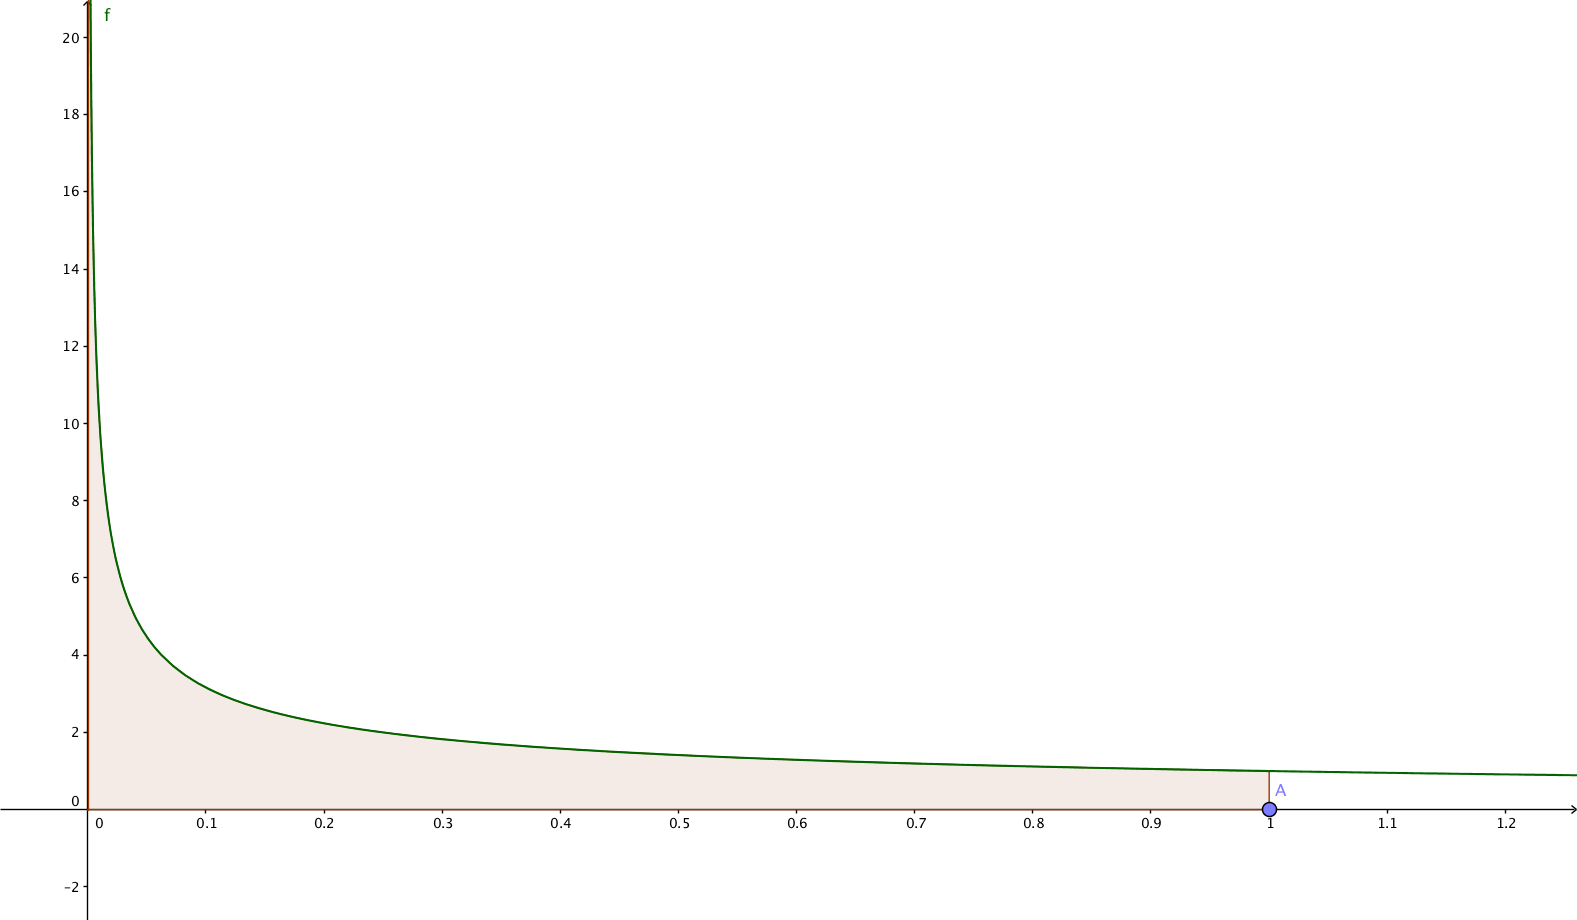
\includegraphics[width=3cm]{integral_uneigentlich}
	\end{example}
\end{frame}

\begin{frame}{Uneigentliche Integrale - Beispiel}	
	\begin{example}
		Die Funktion $f(x)=\frac{1}{x^{2}}=x^{-2}$ konvergiert für $x \to \infty$ gegen $0$.
		Für das (bestimmte) Integral und $a, b \geq 0$ gilt:
		\[
			\int_{a}^{b} \frac{1}{x^2} dx = [ - \frac{1}{x} ]_{a}^{b} =  \frac{1}{a} - \frac{1}{b}
		\]	
		Insbesondere gilt:
		\[
			\int_{1}^{\infty} \frac{1}{x^{2}} dx = \frac{1}{1} - \lim_{b \to \infty}\frac{1}{b} = 1
		\]
	\end{example}
\end{frame}

\begin{frame}{Uneigentliche Integrale - Beispiele}
\begin{example}
\scriptsize{	Die Gammafunktion $\Gamma (x)$, die u.a. in der Statistik eine wichtige Rolle spielt, ist durch das uneigentliche Integral 
	\[
		\Gamma (x) := \int_{0}^{\infty} t^{x-1}e^{-t}\,dt \text{ für } x > 0 
	\]
	definiert.
	Für $\Gamma (x+1)$ erhält man mittels partieller Integration
	\begin{align*}
		\Gamma (x+1) & = \int_{0}^{\infty} t^{x}e^{-t}\, dt = \lim_{b \to \infty} \int_{0}^{b} t^{x}e^{-t}\, dt \\
		& = - \lim_{b \to \infty} \int_{0}^{b} t^{x}(e^{-t})' \, dt \\
		&= - \lim_{b \to \infty} [t^{x}e^{-t}]_{0}^{b} + \int_{0}^{b} (t^{x})' e^{-t}\, dt \\
		&= - \lim_{b \to \infty} b^{x}e^{-b} + \int_{0}^{b} xt^{x-1} e^{-t}\, dt \\
		&= 0 + \lim_{b \to \infty} x\int_{0}^{b} t^{x-1} e^{-t}\, dt = x\Gamma (x)
	\end{align*}
	Wegen $\Gamma (1)=\lim_{b \to \infty} \int_{0}^{b} e^{-t}\,dt = \lim_{b \to \infty} [-e^{-t}]_{0}^{b} = 1$ ist damit 
	\[
	\Gamma (x+1) = x \Gamma (x) = x (x-1) \Gamma(x-2) = x (x-1) (x-2) \ldots 2 \cdot 1 = x!
	\]}
\end{example}
\end{frame}

\subsection{Anwendungen der Integralrechnung}
\subsubsection{Länge von Kurven}
\begin{frame}{Längenberechnung von Kurven}
\begin{definition}
	Für die Länge einer durch eine Funktion $f(x)$ gegebene Kurve zwischen den Stellen $a$ und $b$ gilt:
	\[
		s_{a}^{b}(f) = \int_{a}^{b} \sqrt{1+(f'(x))^{2}}\, dx  
	\]
\end{definition}
\end{frame}

\begin{frame}{Längenberechnung von Kurven - Beispiel}
\begin{example}
\small{	Für die Länge eines Halbkreises mit Radius $R$, der durch die Funkion $f(x)=\sqrt{R^2-x^2}$ dargestellt werden kann, gilt:
	\begin{align*}
		s_{-R}^{R}(f) & = \int_{-R}^{R} \sqrt{1+(f(x)')^{2}}\, dx \\
		& = \int_{-R}^{R} \sqrt{1+\left( -\frac{x}{\sqrt{R^2-x^2}} \right)^{2}}\, dx \\
		& = \int_{-R}^{R} \sqrt{1+\frac{x^2}{R^2-x^2}}\, dx = \int_{-R}^{R} \sqrt{\frac{R^2}{R^2-x^2}}\, dx \\
		& = \int_{-R}^{R} \frac{R}{\sqrt{R^2-x^2}}\, dx = \left[ R \arcsin \frac{x}{R} \right]_{-R}^{R} \\
		& = 2 R \arcsin(1) = R \pi	
	\end{align*}}
\end{example}
\end{frame}

\subsubsection{Rotationskörper}
\begin{frame}{Volumen von Rotationskörpern}
\begin{definition}
	Für die Volumen eines durch Rotation einer Funktion $f(x)$ zwischen den Stellen $a$ und $b$ berandeten Körpers  gilt:
	\[
		V_{a}^{b}(f) = \pi \int_{a}^{b} (f(x))^{2} \, dx  
	\]
	Für die Mantelfläche desselbe Rotationskörpers gilt:
	\[
		O_{a}^{b}(f) = 2\pi \int_{a}^{b} f(x) \sqrt{1+(f'(x))^2}\, dx
	\]
\end{definition}
\end{frame}

\begin{frame}{Rotationskörper - Beispiel}
\small{	\begin{example}
		Ein Kegelstumpf der Höhe $h$ und mit den Deckelradien $r$ und $R$ kann beschrieben werden durch Rotation der linearen Funktion $f(x)= \frac{R-r}{h} \cdot x + r$ um die x-Achse (für $a=0$ und $b=h$ gilt dann $f(a)=f(0)=r$ und $f(b)=f(h)=R$).
		Für das Volumen des Kegelstumpfes gilt dann
		\begin{align*}
			V & = \pi \int_{0}^{h} \left( f(x) \right)^2 \, dx \\
			& = \pi \int_{0}^{h} \left( \frac{R-r}{h} x +r \right)^{2}\, dx \\
			& = \pi \int_{0}^{h} \frac{(R-r)^2}{h^2} x^2  +2 \frac{R-r}{h}xr +r^2 \, dx \\
			& = \pi \left[ \frac{(R-r)^2}{3h^2} x^3  + \frac{R-r}{h}rx^{2} +r^2 x \right]_{0}^{h}\, dx \\
			& = \pi \frac{(R-r)^2}{3}h + (R-r)hr + r^2 h = \frac{h \pi}{3} (R^2 + Rr +r^2 ) 
		\end{align*}
	\end{example}}
\end{frame}

